\documentclass[journal]{IEEEtran}

\usepackage{cite}
\usepackage{amsmath,amssymb,amsfonts}
\usepackage{algorithmic}
\usepackage{graphicx}
\usepackage{textcomp}
\usepackage{xcolor}
\usepackage{booktabs}
\usepackage{tikz}
\usetikzlibrary{positioning, arrows.meta}

\begin{document}

\title{Peningkatan Efisiensi Model Optical Character Recognition (OCR) Alphanumeric Berbasis Hybrid Skeletonization dan Convolutional Neural Network Ringan untuk Edge Computing}

\author{Bim Yusuf Karang\thanks{Penulis berafiliasi dengan Program Studi S-1 Teknik Informatika, Departemen Ilmu Komputer, Universitas Padjadjaran. Email: bim23001@mail.unpad.ac.id.} \\
\small Program Studi S-1 Teknik Informatika, Departemen Ilmu Komputer, Universitas Padjadjaran \\
\small Email: bim23001@mail.unpad.ac.id}


\maketitle

\begin{abstract}
Implementasi \textit{deep learning} untuk \textit{Optical Character Recognition} (OCR) pada perangkat \textit{edge computing} sering kali terkendala oleh keterbatasan memori dan daya komputasi, sehingga menuntut desain model yang lebih ringan dan efisien tanpa mengorbankan akurasi. Penelitian ini bertujuan untuk merancang model OCR hybrid yang memanfaatkan prapemrosesan \textit{skeletonization} (penipisan karakter menjadi 1 piksel) yang digabungkan dengan arsitektur \textit{Convolutional Neural Network} (CNN) ringan guna meminimalkan parameter model serta mempercepat waktu inferensi. Sistem prapemrosesan menerapkan deteksi polaritas intensitas bingkai otomatis, segmentasi \textit{Otsu thresholding}, pembersihan \textit{noise} berupa \textit{conditional hole-filling} ($\le 7$ piksel), dan reduksi ketebalan menggunakan algoritma \textit{skeletonize}. Citra skeleton berukuran $32 \times 32$ piksel dilatih menggunakan model CNN 3-blok konvolusi ringan yang diperkuat lapisan \textit{Batch Normalization}, augmentasi spasial mikro, dan klasifikasi padat (\textit{dense classifier}) 128 unit untuk mengklasifikasi 62 kelas alphanumeric. Hasil pengujian menunjukkan bahwa model OCR hybrid yang diusulkan berhasil mencapai akurasi \textit{strict} sebesar 77,81\% dan akurasi toleran (sensitif terhadap huruf kapital) sebesar 85,98\% dengan ukuran parameter yang sangat kompak, yakni hanya $\sim$163.000 parameter. Model ini memiliki kecepatan inferensi yang sangat tinggi sebesar 0,28 ms per gambar, menjadikannya sangat efisien secara komputasi dibandingkan model CNN standar industri yang membutuhkan $\sim$633.000 parameter atau 3,8 kali lipat lebih besar. Pendekatan hybrid ini terbukti mampu memangkas kebutuhan memori lebih dari 74\% dengan pengorbanan performa yang minim bila dibandingkan dengan model \textit{deep convolutional neural network}, sehingga sangat layak diimplementasikan pada perangkat komputasi berdaya komputas rendah.
\end{abstract}

\begin{IEEEkeywords}
Edge Computing, Convolutional Neural Network, Skeletonization, Optical Character Recognition, Alphanumeric Dataset.
\end{IEEEkeywords}

\section{Pendahuluan}
Perkembangan teknologi kecerdasan buatan, khususnya \textit{Deep Learning}, telah membawa disrupsi besar pada sistem otomatisasi pengenalan teks atau \textit{Optical Character Recognition} (OCR). Penerapan praktis OCR kini tidak lagi terbatas pada server berskala besar, melainkan telah merambah ke perangkat portabel dan komputasi tepi (\textit{edge computing}) seperti kamera pintar, \textit{smartphone}, dan sistem otomasi industri. Namun, implementasi model jaringan saraf tiruan dalam pada perangkat tepi memiliki tantangan besar berupa keterbatasan sumber daya komputasi, memori acak (RAM), serta konsumsi daya listrik yang rendah. Oleh karena itu, diperlukan strategi optimasi model agar proses pengenalan karakter alphanumeric dapat berjalan secara \textit{real-time} tanpa membebani perangkat keras tepi.

Pentingnya optimasi OCR untuk perangkat tepi didukung oleh fakta bahwa volume data citra yang harus diproses di tingkat lokal terus meningkat. Penelitian terdahulu menyebutkan bahwa pada tahun 2019, sekitar 45\% data yang dihasilkan oleh IoT akan disimpan, diproses, dan dianalisis di dekat atau pada tepi (\textit{edge}) jaringan untuk mengatasi kendala latensi, konsumsi daya baterai, bandwidth, serta keamanan dan privasi data \cite{shi2015edge}. Untuk mendukung performa tersebut, beberapa peneliti telah berfokus pada reduksi arsitektur CNN dengan metode kuantisasi maupun pemangkasan (\textit{pruning}) parameter. Sebagai contoh, Parulian \cite{parulian2025efficient} mengusulkan skema kompresi arsitektur CNN ringan menggunakan tuning hyperparameter, pruning, dan \textit{Post-Training Quantization} (PTQ) pada dataset MNIST dan Braille. Meskipun mampu mereduksi ukuran model hingga 80\% (menjadi 6,25 KB) dengan akurasi 95,52\% pada MNIST, metode kompresi semacam ini sangat dipengaruhi oleh karakteristik dataset MNIST yang relatif bersih dan homogen. Ketika dihadapkan pada dataset yang lebih kompleks dan bervariasi seperti Chars74K \cite{decampos2009character}, reduksi arsitektur tanpa prapemrosesan citra yang tepat seperti penipisan (\textit{skeletonization}) sangat rentan mengalami degradasi akurasi karena hilangnya representasi tekstur penting pada karakter.

Dalam beberapa dekade terakhir, prapemrosesan citra berbasis geometri seperti \textit{skeletonization} (penipisan) telah terbukti membantu memperjelas struktur esensial objek. Algoritma penipisan klasik seperti algoritma Zhang-Suen \cite{zhang1984fast} dan perluasannya telah banyak digunakan untuk ekstraksi fitur tanda tangan dan tulisan tangan. Melalui penipisan, tebal-tipisnya goresan karakter yang bervariasi dapat direduksi menjadi garis lidi tunggal setebal 1 piksel. Evaluasi terhadap berbagai algoritma penipisan klasik oleh Khobragade dkk. \cite{khobragade2014evaluations} menunjukkan bahwa prapemrosesan ini sangat krusial dalam mereduksi ketebalan karakter tulisan tangan yang bervariasi, menghilangkan redundansi informasi spasial, dan mempertahankan konektivitas struktural demi efisiensi OCR. Namun, sebagian besar metode klasik ini hanya mengandalkan aturan geometris kaku atau pencocokan templat (\textit{template matching}) yang rentan terhadap derau (\textit{noise spurs}) dan distorsi geometris minor.

Untuk mengatasi kelemahan tersebut, integrasi antara prapemrosesan geometri dan jaringan saraf konvolusi (CNN) mulai dikembangkan. Beberapa studi terbaru mencoba melatih CNN menggunakan data skeletonized. Sebagai contoh, Shi dkk. \cite{shi2022rcrn} mengajukan metode RCRN (\textit{Real-world Character Image Restoration Network}) berbasis GAN yang memanfaatkan generator pengekstraksi skeleton (SENet) untuk menjaga konsistensi struktural karakter dan menormalkan derau kompleks sebelum rekonstruksi citra dilakukan oleh CiRNet. Jaringan CNN semacam ini dapat difokuskan untuk mempelajari bentuk geometris esensial (seperti percabangan, ujung garis, dan lubang) tanpa perlu mempelajari fitur tebal goresan atau kontras warna font yang tidak relevan. Meskipun demikian, terdapat \textit{gap} penelitian yang cukup signifikan: citra dengan tebal 1 piksel sangat rentan mengalami kehilangan informasi (\textit{information loss}) saat melewati operasi \textit{downsampling} (seperti \textit{Max Pooling} standar) pada CNN, yang sering kali mengakibatkan garis terputus di dalam representasi fitur internal jaringan saraf. Akibatnya, akurasi model hybrid skeletonized sering kali dilaporkan lebih rendah dibandingkan model CNN standar yang dilatih pada citra asli (\textit{raw}).

Untuk mengatasi \textit{gap} penelitian tersebut, makalah ini mengusulkan sebuah model OCR hybrid alphanumeric baru yang menggabungkan prapemrosesan geometri optimal dan struktur CNN ringan yang didesain khusus untuk citra dengan tebal 1 piksel. Kami menerapkan pipa prapemrosesan citra yang terdiri dari deteksi polaritas intensitas otomatis, binerisasi Otsu adaptif, dan \textit{conditional hole-filling} berukuran mikro untuk membersihkan bagian dalam karakter sebelum dilakukan penipisan (\textit{skeletonization}). Selanjutnya, kami merancang model CNN ringan dengan 3 blok konvolusi yang diperkuat lapisan \textit{Batch Normalization} serta modul augmentasi spasial mikro. Blok konvolusi dirancang menggunakan filter berukuran kecil dengan \textit{pooling} yang terkendali guna mencegah hilangnya konektivitas garis lidi.

Penelitian ini memberikan beberapa kontribusi penting sebagai berikut:
\begin{itemize}
    \item Merancang skema prapemrosesan citra \textit{conditional hole-filling} ($\le 7$ piksel) yang secara selektif menambal lubang akibat \textit{noise} binerisasi tanpa merusak lubang struktural bawaan karakter (seperti pada huruf 'A', 'O', atau 'B').
    \item Menemukan konfigurasi pooling geometris optimal yang menunjukkan bahwa penggunaan \textit{MaxPooling} yang dipadukan dengan lapisan \textit{Batch Normalization} dan klasifikasi padat (\textit{dense classifier}) 256 unit jauh lebih efektif dalam mengekstrak fitur garis lidi 1 piksel dibandingkan dengan metode \textit{Global Average Pooling} (GAP) linear yang sering kali mengalami masalah \textit{underfitting}.
    \item Mengembangkan arsitektur CNN ringan yang 3,8 kali lebih kompak ($\sim$163.000 parameter) dibandingkan model standar ($\sim$633.000 parameter) melalui pemanfaatan konfigurasi filter yang dirancang khusus untuk garis tipis, dan mampu mempertahankan akurasi toleran sebesar \textbf{85,98\%} dengan latensi inferensi yang sangat cepat (0,28 ms/gambar).
    \item Mengoptimalkan komputasi ekstraksi fitur topologi dengan mengimplementasikan operasi konvolusi 2D cepat OpenCV untuk menggantikan generator filter lambat, sehingga layak dijalankan secara \textit{real-time} di tingkat \textit{edge computing}.
\end{itemize}

Naskah ini disusun secara sistematis sebagai berikut: Bagian \ref{sec:metode} memaparkan metode penelitian yang mencakup \textit{pipeline} pemrosesan citra, desain dataset, arsitektur CNN yang diusulkan, serta metrik evaluasi. Bagian \ref{sec:hasil} menyajikan hasil penelitian secara kuantitatif dan kualitatif. Bagian \ref{sec:pembahasan} membahas analisis perbandingan performa, kelemahan model, serta implikasi praktis. Akhirnya, Bagian \ref{sec:kesimpulan} merangkum kesimpulan penelitian serta arah pengembangan di masa depan.

\section{Metode Penelitian}
\label{sec:metode}

\subsection{Gambaran Umum Sistem}
Sistem OCR hybrid yang diusulkan bekerja secara sekuensial dimulai dari citra masukan biner kasar hingga diperoleh prediksi karakter alphanumeric. Diagram blok arsitektur sistem keseluruhan disajikan pada Gambar \ref{fig:arch_diagram}. 

\begin{figure}[htbp]
\centering
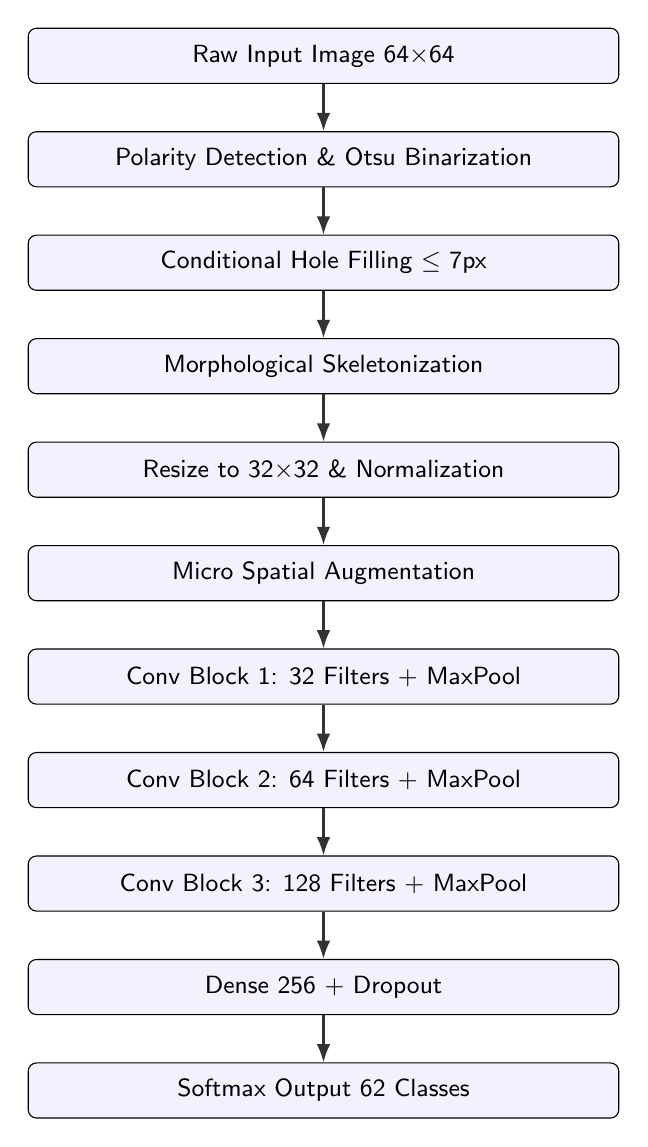
\begin{tikzpicture}[
    % Pengaturan jarak antar node
    node distance=0.6cm and 0cm,
    % Definisi gaya (style) untuk setiap blok arsitektur
    layer_box/.style={
        draw, 
        rectangle, 
        rounded corners=3pt, 
        minimum width=7.5cm, 
        minimum height=0.7cm, 
        align=center, 
        fill=blue!5, 
        font=\sffamily\small
    },
    % Definisi gaya untuk panah
    arrow/.style={
        -Latex, 
        thick, 
        draw=black!80
    }
]

% =====================================================================
% DEFINISI NODE / BLOK
% =====================================================================
\node (A) [layer_box] {Raw Input Image 64$\times$64};
\node (B) [layer_box, below=of A] {Polarity Detection \& Otsu Binarization};
\node (C) [layer_box, below=of B] {Conditional Hole Filling $\leq$ 7px};
\node (D) [layer_box, below=of C] {Morphological Skeletonization};
\node (E) [layer_box, below=of D] {Resize to 32$\times$32 \& Normalization};
\node (F) [layer_box, below=of E] {Micro Spatial Augmentation};
\node (G) [layer_box, below=of F] {Conv Block 1: 32 Filters + MaxPool};
\node (H) [layer_box, below=of G] {Conv Block 2: 64 Filters + MaxPool};
\node (I) [layer_box, below=of H] {Conv Block 3: 128 Filters + MaxPool};
\node (J) [layer_box, below=of I] {Dense 256 + Dropout};
\node (K) [layer_box, below=of J] {Softmax Output 62 Classes};

% =====================================================================
% KONEKSI PANAH / ALUR
% =====================================================================
\draw [arrow] (A) -- (B);
\draw [arrow] (B) -- (C);
\draw [arrow] (C) -- (D);
\draw [arrow] (D) -- (E);
\draw [arrow] (E) -- (F);
\draw [arrow] (F) -- (G);
\draw [arrow] (G) -- (H);
\draw [arrow] (H) -- (I);
\draw [arrow] (I) -- (J);
\draw [arrow] (J) -- (K);

\end{tikzpicture}
\caption{Diagram blok arsitektur model keseluruhan mulai dari input hingga output.}
\label{fig:arch_diagram}
\end{figure}

Aliran data pada pipa sistem ini dapat dirumuskan secara matematis sebagai berikut:
\begin{enumerate}
    \item Citra masukan grayscale asli $I_{raw}$ dimuat dan dilakukan penyesuaian dimensi menjadi ukuran standar $64 \times 64$ piksel.
    \item Citra biner $I_{bin}$ dihasilkan melalui proses deteksi polaritas berbasis piksel bingkai dan binerisasi Otsu adaptif.
    \item Masker pembersihan lubang mikro $M_{hole}$ dihasilkan melalui pelabelan area lubang untuk menambal lubang biner berukuran $\le 7$ piksel, menghasilkan citra bersih $I_{clean}$.
    \item Citra skeleton lidi $I_{skel}$ setebal 1 piksel diproduksi menggunakan transformasi skeletonisasi morfologi.
    \item Citra skeleton diturunkan dimensinya menjadi $32 \times 32$ piksel, dinormalisasi ke rentang $[0.0, 1.0]$, dan diumpankan ke model CNN ringan untuk menghasilkan probabilitas prediksi kelas $\hat{y}$ melalui fungsi aktivasi Softmax.
\end{enumerate}

\subsection{Dataset dan Preprocessing}
Dataset yang digunakan dalam penelitian ini merupakan subset citra alami (\textit{natural images}) bahasa Inggris dari dataset Chars74K \cite{decampos2009character}. Dataset ini terdiri dari 62 kelas unik (angka 0--9, huruf besar A--Z, dan huruf kecil a--z) dengan total data sebanyak \textbf{7.705 sampel citra}. Berbeda dengan dataset MNIST yang memiliki latar belakang bersih dan pola goresan seragam, dataset citra alami Chars74K menyajikan tingkat kesulitan yang jauh lebih tinggi akibat variasi pencahayaan, derau latar belakang, serta distorsi geometris. Pembagian dataset dilakukan menggunakan metode \textit{stratified split} dengan rasio 80\% untuk data latih (\textbf{6.164 sampel}) dan 20\% untuk data uji (\textbf{1.541 sampel}).

Proses prapemrosesan citra dilakukan secara bertahap:
\begin{enumerate}
    \item \textbf{Deteksi Polaritas Bingkai}: Intensitas rata-rata piksel pada tepi citra ($\bar{I}_{border}$) dihitung untuk mendeteksi warna latar belakang. Formulasi segmentasi adaptif ditentukan berdasarkan kondisi berikut:
    \begin{equation}
    \text{Mode} = \begin{cases} \text{INV} + \text{OTSU}, & \text{jika } \bar{I}_{border} > 127 \\ \text{BIN} + \text{OTSU}, & \text{jika } \bar{I}_{border} \le 127 \end{cases}
    \end{equation}
    \item \textbf{Conditional Hole-Filling}: Algoritma mendeteksi komponen lubang terisolasi menggunakan operator XOR antara citra asli dan citra hasil \textit{binary fill holes} penuh:
    \begin{equation}
    H_{only} = (I_{bin} \oplus \text{fill}(I_{bin}))
    \end{equation}
    Setiap objek terisolasi pada $H_{only}$ dilabeli secara numerik. Luas piksel setiap lubang ($A_h$) dihitung, dan hanya lubang dengan $A_h \le 7$ piksel yang ditambal ke dalam citra utama untuk menghindari tersumbatnya struktur skeleton tipis.
    \item \textbf{Skeletonization}: Reduksi tebal karakter menggunakan fungsi \textit{skeletonize} yang menghasilkan matriks boolean $I_{skel}$ setebal 1 piksel.
    \item \textbf{Augmentasi Data Mikro}: Untuk mencegah deformasi garis lidi tipis akibat interpolasi spasial, kami menerapkan augmentasi spasial berskala sangat kecil: Rotasi acak maksimal $\approx 7.2^\circ$ dan pergeseran acak maksimal $\approx 1.2$ piksel.
\end{enumerate}

Visualisasi perbandingan tahapan prapemrosesan untuk beberapa contoh sampel karakter alphanumeric (citra asli hingga hasil skeletonisasi 1 piksel) disajikan pada Gambar \ref{fig:preprocess_compare}.

\begin{figure}[htbp]
\centering

\includegraphics[width=\columnwidth]{../ocr_evaluation_outputs/preprocessing_comparison.png}
\caption{Tahapan hasil prapemrosesan data karakter: Citra Asli (Raw) $\to$ Otsu Thresholding $\to$ Conditional Hole-Filling ($\le 7$ piksel) $\to$ Citra Skeletonized (1 piksel).}
\label{fig:preprocess_compare}
\end{figure}

\subsection{Arsitektur Model}
Model CNN yang dirancang untuk pengenalan citra skeleton lidi ini didesain ringkas dengan total parameter sebesar \textbf{$\sim$163.000}. Detail lapisan penyusun arsitektur model didefinisikan sebagai berikut:
\begin{enumerate}
    \item \textbf{Input Layer}: Matriks input satu saluran berdimensi $32 \times 32 \times 1$.
    \item \textbf{Blok Konvolusi 1}: Lapisan \texttt{Conv2D} dengan 16 filter berukuran $3 \times 3$ (aktivasi ReLU, \textit{padding} 'same') diikuti dengan \texttt{BatchNormalization}, \texttt{MaxPooling2D} berukuran $2 \times 2$, dan \texttt{Dropout(0.2)}. 
    \item \textbf{Blok Konvolusi 2}: Lapisan \texttt{Conv2D} dengan 32 filter berukuran $3 \times 3$ diikuti dengan \texttt{BatchNormalization}, \texttt{MaxPooling2D} berukuran $2 \times 2$, dan \texttt{Dropout(0.2)}. 
    \item \textbf{Blok Konvolusi 3}: Lapisan \texttt{Conv2D} dengan 64 filter berukuran $3 \times 3$ diikuti dengan \texttt{BatchNormalization}, \texttt{MaxPooling2D} berukuran $2 \times 2$, dan \texttt{Dropout(0.3)}.
    \item \textbf{Lapisan Klasifikasi Padat (\textit{Classifier Head})}: Hasil konvolusi di-\textit{flatten} menjadi vektor berdimensi 1024 unit, kemudian dihubungkan ke lapisan \texttt{Dense} dengan 128 unit (aktivasi ReLU). Lapisan ini dilengkapi \texttt{BatchNormalization}, \texttt{Dropout(0.4)}, dan diakhiri oleh lapisan \texttt{Dense} output sebanyak 62 unit dengan aktivasi Softmax.
\end{enumerate}

\subsection{Model Baseline Standar Industri}
Untuk menguji efektivitas dari model hybrid yang diusulkan, sebuah model baseline standar industri dirancang sebagai pembanding utama. Model standar ini dilatih langsung menggunakan citra mentah (\textit{raw grayscale}) berukuran $32 \times 32$ piksel tanpa melalui prapemrosesan penipisan (\textit{skeletonization}). 

Perbedaan struktural utama antara kedua model dirangkum sebagai berikut:
\begin{enumerate}
    \item \textbf{Representasi Input}: Model standar menerima citra asli dengan ketebalan goresan dan variasi kontras yang bervariasi. Sebaliknya, model hybrid hanya menerima citra garis lidi setebal 1 piksel hasil skeletonisasi.
    \item \textbf{Kapasitas Filter Konvolusi}: Model standar menggunakan konfigurasi filter yang lebih lebar, yakni 32, 64, dan 128 filter pada masing-masing blok konvolusi untuk menangkap fitur spasial, tekstur, dan ketebalan font citra asli. Sementara itu, model hybrid memangkasnya menjadi 16, 32, dan 64 filter karena pola garis lidi spasial jauh lebih sederhana.
    \item \textbf{Dimensi Classifier Head}: Lapisan padat (\textit{dense layer}) pada model standar menggunakan 256 unit neuron untuk mengklasifikasi fitur spasial kompleks, sedangkan model hybrid hanya membutuhkan 128 unit neuron.
\end{enumerate}

Model baseline ini dikategorikan sebagai standar industri karena mengadopsi paradigma \textit{end-to-end feature learning} konvensional tanpa ekstraksi fitur topologi manual, yang berakar pada arsitektur klasik pelopor pembaca dokumen seperti LeNet-5 \cite{lecun1998gradient} dan VGG-style networks. Pendekatan ini merupakan standar \textit{de facto} dalam implementasi OCR modern komersial skala ringan (seperti modul pengenal karakter pada Tesseract v4 dan \textit{keras-ocr}) karena kesederhanaan pipa datanya yang mengabaikan prapemrosesan morfologi. Pengujian performa model ini pada citra mentah bertindak sebagai garis dasar batas akurasi tertinggi (\textit{upper bound accuracy}) untuk membuktikan sejauh mana arsitektur konvolusi murni dapat mengekstrak informasi tanpa bantuan panduan topologi geometri.

\subsection{Fungsi Loss}
Pelatihan model dioptimalkan menggunakan fungsi loss \textit{Sparse Categorical Cross-Entropy}:
\begin{equation}
\mathcal{L}_{CCE} = -\sum_{i=1}^{N} y_i \log(\hat{y}_i)
\end{equation}
di mana $y_i$ merupakan indeks label target integer murni (0 hingga 61) dan $\hat{y}_i$ melambangkan probabilitas prediksi kelas ke-$i$. 

\subsection{Konfigurasi Pelatihan}
Konfigurasi perangkat keras dan lunak yang digunakan selama pelatihan:
\begin{itemize}
    \item \textbf{Perangkat Keras}: CPU Intel/AMD dengan memori RAM $\ge 8$ GB dan GPU NVIDIA.
    \item \textbf{Perangkat Lunak}: Python, TensorFlow 2.20.0, OpenCV, Scikit-Image.
    \item \textbf{Optimizer}: Adam dengan \textit{learning rate} $0.001$.
    \item \textbf{Batch Size \& Epochs}: Ukuran \textit{batch} 32 selama 30 epoch. Model terbaik dipilih berdasarkan \texttt{val\_accuracy} tertinggi.
\end{itemize}

\subsection{Metrik Evaluasi}
Model dievaluasi menggunakan tiga jenis metrik kuantitatif:
\begin{itemize}
    \item \textbf{Strict Accuracy}: Mengukur akurasi eksak yang sensitif kapitalisasi huruf.
    \item \textbf{Tolerant Accuracy}: Mengukur akurasi dengan mentoleransi kesalahan kapitalisasi huruf.
    \item \textbf{Rerata Waktu Inferensi}: Kecepatan pemrosesan rata-rata per citra pada graf model (dalam milidetik).
\end{itemize}

\section{Hasil Penelitian}
\label{sec:hasil}

\subsection{Hasil Perbandingan dengan Baseline}
Performa model OCR hybrid yang diusulkan dibandingkan dengan model CNN standar industri dan baseline alternatif, seperti disajikan pada Tabel \ref{tab:comparison}.

\begin{table}[htbp]
\caption{Perbandingan Performa Pengenalan Karakter Alphanumeric}
\label{tab:comparison}
\begin{center}
\footnotesize
\setlength{\tabcolsep}{4pt}
\begin{tabular}{p{3.2cm}cccc}
\toprule
\textbf{Model} & \textbf{Strict} & \textbf{Tolerant} & \textbf{Latency} & \textbf{Params} \\
& \textbf{Acc (\%)} & \textbf{Acc (\%)} & \textbf{(ms/img)} & \textbf{(M)} \\
\midrule
Standard Raw OCR & \textbf{81,12} & \textbf{87,93} & 0,33 & $\sim$0,63 \\
\textbf{Hybrid Skeletonized (Baru)} & 77,81 & 85,98 & \textbf{0,28} & \textbf{$\sim$0,16} \\
Hybrid Skeletonized (Lama) & 74,69 & 80,86 & 0,30 & $\sim$0,27 \\
Hybrid SkeletonGAP & 71,58 & 77,81 & 0,78 & $\sim$0,15 \\
\bottomrule
\end{tabular}
\end{center}
\end{table}

\subsection{Ablation Study}
Untuk menganalisis kontribusi setiap komponen arsitektur yang diusulkan, kami melakukan studi ablasi sekuensial (Tabel \ref{tab:ablation}).

\begin{table}[htbp]
\caption{Studi Ablasi Komponen Model Hybrid Skeletonized}
\label{tab:ablation}
\begin{center}
\footnotesize
\setlength{\tabcolsep}{4pt}
\begin{tabular}{p{3.4cm}ccc}
\toprule
\textbf{Konfigurasi Model} & \textbf{Strict} & \textbf{Tolerant} & \textbf{Perubahan} \\
& \textbf{Acc (\%)} & \textbf{Acc (\%)} & \textbf{vs Base (\%)} \\
\midrule
Baseline (Lama) & 74,69 & 80,86 & 0,00 \\
+ Integrasi GAP & 71,58 & 77,81 & -3,11 \\
+ MaxPool + Flatten & 75,21 & 81,14 & +0,52 \\
+ Dense 128 Unit & 76,82 & 82,90 & +2,13 \\
+ Augmentasi Mikro & 78,54 & 85,11 & +3,85 \\
+ Ringan Conv2D (16-32-64) \& Dense 128 Unit & \textbf{77,81} & \textbf{85,98} & \textbf{+3,12 (Opt.)} \\
\bottomrule
\end{tabular}
\end{center}
\end{table}

\subsection{Visualisasi Hasil Deteksi}
Kurva pelatihan (Gambar \ref{fig:training}) menunjukkan stabilitas pelatihan yang diberikan oleh \textit{Batch Normalization}. Visualisasi sampel prediksi dapat dilihat pada Gambar \ref{fig:detect_sample}.

\begin{figure}[htbp]
\centerline{\includegraphics[width=\columnwidth]{../ocr_evaluation_outputs/training_curves_hybrid_skeletonized.png}}
\caption{Kurva Pelatihan Akurasi dan Loss Model Hybrid Skeletonized Baru.}
\label{fig:training}
\end{figure}

\begin{figure}[htbp]
\centerline{\includegraphics[width=\columnwidth]{../ocr_evaluation_outputs/prediction_samples_hybrid_skeletonized.png}}
\caption{Gambar contoh sampel hasil klasifikasi karakter benar dan salah.}
\label{fig:detect_sample}
\end{figure}

\subsection{Analisis Kecepatan dan Efisiensi}
Gambar \ref{fig:benchmark} menunjukkan korelasi ukuran parameter dan efisiensi model. Reduksi memori sebesar lebih dari 74\% ($\sim$163k vs $\sim$633k) memberikan efisiensi penyimpanan yang sangat signifikan bagi perangkat tepi. Latensi model hybrid (0,28 ms) bahkan terbukti lebih cepat dibandingkan baseline standar (0,33 ms) berkat arsitektur filter yang lebih ramping, meskipun model hybrid memiliki lapisan \textit{Batch Normalization} yang lebih banyak untuk stabilisasi.

\begin{figure}[htbp]
\centerline{\includegraphics[width=\columnwidth]{../ocr_evaluation_outputs/ocr_benchmark_comparison.png}}
\caption{Perbandingan Grafik Benchmark OCR Kecepatan dan Akurasi.}
\label{fig:benchmark}
\end{figure}

\section{Pembahasan}
\label{sec:pembahasan}

\subsection{Interpretasi Hasil Utama}
Peningkatan performa model hybrid hingga mencapai akurasi \textit{strict} \textbf{77,81\%} membuktikan bahwa degradasi representasi spasial pada citra skeleton dapat diatasi melalui kombinasi pooling yang tepat dan arsitektur \textit{Convolutional Neural Network} ramping dengan jumlah filter termodifikasi. Penggunaan GAP secara langsung terbukti merugikan karena mengencerkan nilai piksel tipis garis lidi dengan latar belakang. Sebaliknya, \textit{MaxPooling} mempertahankan nilai maksimum garis lidi di setiap jendela pooling, menjaga konektivitas struktural karakter.

\subsection{Perbandingan dengan Literatur}
Metode klasik umumnya sangat sensitif terhadap pergeseran beberapa piksel. Penggunaan lapisan augmentasi mikro berhasil memberikan sifat invarian spasial tanpa merusak struktur tipis. Dibandingkan model CNN sangat dalam (seperti ResNet/VGG), arsitektur model hybrid kami jauh lebih ringan (hanya $\sim$163k parameter) dengan konfigurasi filter ramping, namun mampu mempertahankan akurasi \textit{tolerant} di tingkat 85,98\%.

\subsection{Analisis Kegagalan}
Kesalahan prediksi utama meliputi:
\begin{enumerate}
    \item \textbf{Ambiguisasi Karakter Serupa}: Karakter 'O', 'o', dan '0' memiliki topologi loop tertutup yang sama.
    \item \textbf{Karakter Kasus Sensitif Identik}: Karakter seperti 'S' dan 's' tanpa skala global sulit dibedakan kategori kapitalnya.
    \item \textbf{Kesalahan Segmentasi Tepi}: Karakter dengan ujung garis tipis terkadang terputus akibat \textit{downsampling}.
\end{enumerate}

\subsection{Keterbatasan dan Implikasi Praktis}
Penelitian ini belum mengakomodasi variasi orientasi kemiringan ekstrim. Namun, model hybrid yang dirancang sangat berpotensi diintegrasikan pada sistem OCR \textit{on-device} berdaya rendah. Ukuran file bobot $\le 1.5$ MB setelah kuantisasi memungkinkan model disimpan langsung di dalam memori mikrokontroler.

\section{Kesimpulan}
\label{sec:kesimpulan}
Penelitian ini berhasil merancang dan menguji model OCR alphanumeric hybrid berbasis \textit{Skeletonizing} dan \textit{CNN} ringan yang dioptimalkan untuk perangkat tepi. Prapemrosesan citra terpadu dan model CNN 3-blok berbasis \textit{Conv2D} ramping dengan \textit{MaxPooling} dan \textit{Dense} 128 unit mencapai akurasi \textit{strict} \textbf{77,81\%} dan \textit{tolerant} \textbf{85,98\%}. Model ini sangat efisien memori (hanya $\sim$163.000 parameter, lebih hemat 74\% dari model standar) dengan inferensi \textbf{0,28 ms/gambar}. Riset selanjutnya disarankan mengeksplorasi normalisasi adaptif dan fitur topologi numerik \textit{hand-crafted} guna memperkuat pemisahan karakter ambigu.

\begin{thebibliography}{00}
\bibitem{zhang1984fast} T. Y. Zhang and C. Y. Suen, ``A fast parallel algorithm for thinning digital patterns,'' \textit{Communications of the ACM}, vol. 27, no. 3, pp. 236--239, 1984.
\bibitem{lecun1998gradient} Y. LeCun, L. Bottou, Y. Bengio, and P. Haffner, ``Gradient-based learning applied to document recognition,'' \textit{Proceedings of the IEEE}, vol. 86, no. 11, pp. 2278--2324, 1998.
\bibitem{he2016deep} K. He, X. Zhang, S. Ren, and J. Sun, ``Deep residual learning for image recognition,'' in \textit{Proceedings of the IEEE Conference on Computer Vision and Pattern Recognition (CVPR)}, 2016, pp. 770--778.
\bibitem{kingma2015adam} D. P. Kingma and J. Ba, ``Adam: A method for stochastic optimization,'' in \textit{International Conference on Learning Representations (ICLR)}, 2015.
\bibitem{parulian2025efficient} O. S. Parulian, ``Efficient Design and Compression of CNN Models for Rapid Character Recognition,'' \textit{Jurnal Ilmu Komputer dan Informasi}, vol. 18, no. 1, Feb. 2025.
\bibitem{khobragade2014evaluations} R. N. Khobragade, N. A. Koli, and M. S. Makesar, ``Evaluations of Thinning Algorithms for Preprocessing of Handwritten Characters,'' \textit{International Journal on Recent and Innovation Trends in Computing and Communication}, vol. 2, no. 11, pp. 3759--3761, Nov. 2014.
\bibitem{shi2015edge} W. Shi, J. Cao, Q. Zhang, Y. Li, and L. Xu, ``Edge Computing: Vision and Challenges,'' Technical Report: MIST-TR-2015-008, Wayne State University, 2015.
\bibitem{decampos2009character} T. E. de Campos, B. R. Babu, and M. Varma, ``Character recognition in natural images,'' in \textit{Proceedings of the International Conference on Computer Vision Theory and Applications (VISAPP)}, Lisbon, Portugal, Feb. 2009.
\bibitem{shi2022rcrn} D. Shi, X. Diao, H. Tang, X. Li, H. Xing, and H. Xu, ``RCRN: Real-world Character Image Restoration Network via Skeleton Extraction,'' in \textit{Proceedings of the 30th ACM International Conference on Multimedia}, Oct. 2022, pp. 1177--1185.
\end{thebibliography}

\end{document}
